
\documentclass[letterpaper, 10 pt, conference]{ieeeconf}  % Comment this line out if you need a4paper
%\documentclass[a4paper, 10pt, conference]{ieeeconf}      % Use this line for a4 paper

\IEEEoverridecommandlockouts  % This command is only needed if you want to use the \thanks command
\overrideIEEEmargins
% See the \addtolength command later in the file to balance the column lengths
% on the last page of the document



% The following packages can be found on http:\\www.ctan.org
\usepackage{graphics} % for pdf, bitmapped graphics files
\usepackage{graphicx}
%\usepackage{epsfig} % for postscript graphics files
%\usepackage{mathptmx} % assumes new font selection scheme installed
%\usepackage{times} % assumes new font selection scheme installed
\usepackage{amsmath} % assumes amsmath package installed
\usepackage{amssymb}  % assumes amsmath package installed
\usepackage{hyperref}

\title{\Huge 
Network Tomography of Cortical Neuronal Molecular Communication Systems
}

\author{Peter Mullen, Dr. Nicola Marchetti, Dr. Michael Barros}

\begin{document}

\maketitle
\thispagestyle{empty}
%\pagestyle{empty}
\pagestyle{plain} 

\begin{abstract}
With the proposal of numerous brain-machine interfaces offering data measurement
of cortical information through minimally-invasive means comes the need for a better
understanding of the circuit-level characteristics of these neuronal systems. These
devices allow data access at a level that can bridge the gap between biological
neuronal analysis and classical communication theory that has been developed for
and applied to man-made network systems. 
In this paper we study the application of classical communication theory in the
biological domain, investigating how network tomography could be
achieved with cortical neuronal circuits. This work involves the simulation of
various neuronal circuits, extraction of the simulated data, and the analysis of this data to develop a
classifying model to infer internal network characteristics based on the measured
endpoint data. Through the processing of the observed data into probabilistic models, we investigate
the use of information theory in cell-to-cell links, and find limitations in the application of
digital mutual information analysis in the biological domain. We investigate the use of simple cross-correlation methods for estimating the synaptic delay in a neuronal circuit, achieving a correlative R-squared score of 0.55.
We also separately train a support-vector machine classifier to identify
the specific cell type (and sub-group types) from input-output voltage measurements, achieving accuracies of up to 70\%.
This research can help to advance the next generation of brain-machine interfaces by improving our current understanding of these circuits and the constraints that may come with the application of existing telecommunicative theories in the biological domain.\\
\textit{Index Terms} - Brain goo
\end{abstract}



\section{INTRODUCTION}
Several brain-machine interfaces have been proposed in recent years which aim to offer measurement of cortical information through minimally-invasive means. With the introduction of such data measurement techniques comes the need to further our understanding of the circuit-level characteristics of these neuronal systems such that the available data can be adequately utilised. The devices will allow access to information of neuronal networks at a level similar to that available from the analysis of man-made network systems, bridging the gap between biological neuronal analysis and classical communication theory that has been developed for (and applied to) these existing network systems such as those discussed in \cite{mBarrosMolCom}.\\
The main aim of this project is to investigate the application of existing communication theory in the biological and neuronal domain, specifically in cortical neuronal circuits. Building a model based on this existing theory and machine learning techniques, we aim to infer internal network characteristics and classify cell types from limited endpoint data which could be measured through minimally-invasive approaches in the future, such as the Neural Dust discussed in \cite{NeurDust} by researchers in the University of Berkeley. While these physical data measurement techniques are not yet mature enough to be used in practice, existing tools such as the NEURON simulation software from Yale can generate accurate simulated data based on known cell types, similar to the form of data which will be measurable by the aforementioned physical devices. The data obtained from this software can then be processed through mathematical software such as Matlab or data-mining software such as RapidMiner, which offers a powerful environment for developing data processing and machine learning models. By integrating and defining an interface between NEURON, Matlab, and RapidMiner, we obtain the framework needed to simulate the communication between biological neurons and to analyse it through machine learning techniques.\\
One of the primary goals of this project is to investigate the classification and inference of neuronal circuits, especially at an inter-layer scale and with a larger variety of cell-types, progressing the field towards classification of more complex cortical circuits.\\
We investigate the effect of signal propagation in the circuits, and attempt to quantise the level of information communicated between cells. The data generated by the NEURON tool represents the signals as they exist in an ideal network, and so we investigate the effects that cell-to-cell connection parameters may have on the ability for the cells to transfer information between each other. To this end, we investigate the application of digital forms of information theoretic models in the biological domain, and find limitations in the insight that these models may provide in this setting.\\
We also investigate the use of classification algorithms in the analysis of various forms of cortical networks from known networks such as those discussed in \cite{bbpTop}. One requirement in the use of such classifiers is the need to reduce the dimensionality of the measured data. This is done through feature extraction, which can also be applied to the neural network and decision tree models to improve performance. We therefore attempt to characterise the response of individual neural cells in a finite dimension space uisng the Linear-Nonlinear-Poisson cascade model. Through the use of characteristic models and integration with various classification algorithms, we develop a classification system to predict cell type (and sub-group type) based entirely off input-output voltage measurements.\\
Finally, we investigate the use of the classification models trained on the data from the previous step in the application of network tomography to reconstruct the cell-types in a known topology based on endpoint measurements taken around the network.\\
TODO: Paper outline

\section{NEURONS AND NEURONAL CHARACTERISATION}

Neurons are a class of cell present in the body of most multicellular organisms, differentiated from other biological cells by their ability to be stimulated by an electrical signal, responding in kind with an electrical signal which can be used to excite further neurons. Neuronal cells with varying roles work together to form the nervous system which allow the organism to have contextual awareness of the environment. While different neurons may have separate roles in the body, the basic form of each neuron is typically made of three sections: the branched system of dendrites acting as input to the cell, the soma (cell body) which houses the cell nucleus, and an axon acting as cell output, delivering the signal to the dendrites of one or more subsequent cells. Typically, the axon and subsequent dendrite of a cell-to-cell connection are not directly connected, rather the electrical signal is passed through an electro-chemical interface referred to as a \emph{synapse}. For a given synaptic connection, the neuron acting as a signal source is referred to as the \emph{pre-synaptic cell} while the neuron acting as the signal receiver is referred to as the \emph{post-synaptic cell}.\\
The arrival of a signal at the pre-synaptic axon terminal of the synapse triggers the release of \emph{neurotransmitters}, a class of chemical which travels across the synapse and binds to a receptor at the dendritic receiver causing some form of electrical response in the post-synaptic cell. Due to the nature of this method of signal propagation, different synapses may have varying degrees of electrical-response characteristics; for example, there may be a refractory period following the propagation of a signal during which subsequent signals will not be propagated due to the temporary depletion of available neurotransmitters in the synapse. \\
In this study, we deal solely with the neurons found in the brain; specifically, the neurons investigated are based on prior research into the neurons of the somatosensory cortex of a juvenile rat. This segment is found in the the outer portion of the cerebrum of the brain, referred to as the neocortex. The neocortex is typically treated as being a tightly-packed system of vertical structures (cortical columns), and classified into 6 interconnected horizontal layers, referred to as L1-L6 (with layers 2 and 3 often grouped together and referred to as L2/3). Neurons are also classified by morphological-type (m-type) which defines the physical shape and layout of the neuron, and by electrical type (e-type) which defines the electrical characteristics of the cell. The neurons in this investigation are based on data retrieved from a single cortical column, each classified by layer, m-type, and e-type.\\
\begin{figure}[ht]
    \centering
    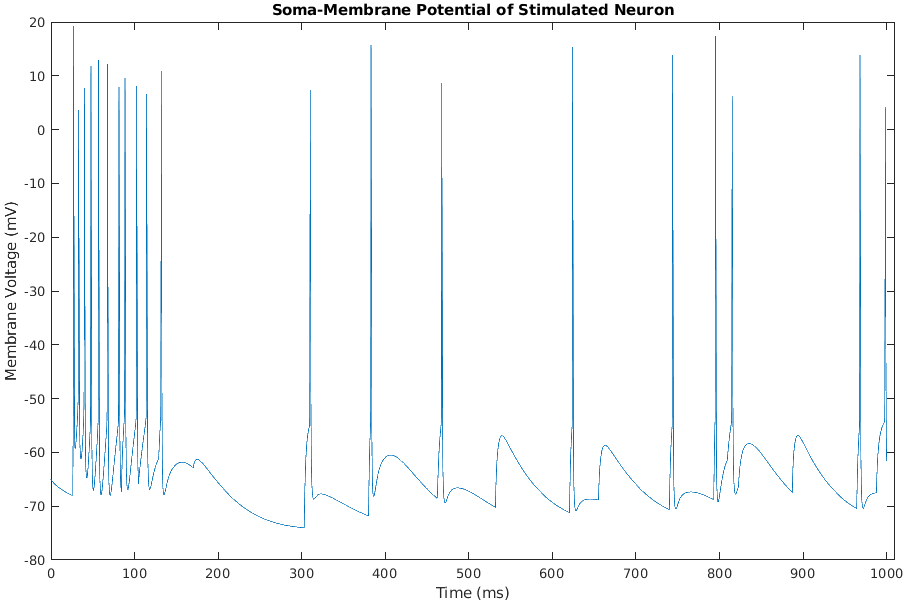
\includegraphics[width=0.48\textwidth]{sampleSpikeTrain.png}
    \caption{Spike Train of a Neural Cell}
    \label{image:sampleSpike}
\end{figure}
\subsection*{Cortical Topologies}
There are two main topologies investigated in this study: 2-cell topology, and 4-leaf star topology. The 2-cell topology consists of two cells linked by a synaptic connection whose parameters vary between network to network. It is quite a simple topology and is used in this study mainly to analyse the link between two neurons rather than to investigate the various effects of neuronal layout. The 4-leaf star topology is a slightly more complex network. The intention of the use of this network is to analyse the application of the results found from the study of the 2-cell networks in more complex topologies to investigate what effects, if any, the topology may have on performance. It is important to note here that the direction of the synaptic connections is that of an "out-hub", i.e. the central node (acting as the hub) is delivering voltage spikes to the surrounding leaves.

\subsection*{Cell Characterisation}
Of major interest to us in this investigation is the characterisation of the response of neurons to a given signal. This response is of the \emph{all-or-none} principle; that is, the cell will either respond fully or will not respond at all. The response takes the form of a voltage spike, and the response over time is characterised as a spike train. A sample time-voltage plot from the measurement of the soma-membrane voltage of a simulated neuron is shown in Figure \ref{image:sampleSpike}. As the release of neurotransmitters in the synapse is a response of a spike event rather than of the small variations in resting potential, the response of a post-synaptic cell is therefore also a function of the spike events. Analytically, the spike events are treated in a probabilistic fashion (i.e. the probability of a spike occurring) to which a Poisson process fits well. The Poisson process describes a model for the estimated time between events, and so when applied in this domain to estimate the time between voltage spikes, the intercellular signals are seen as a \emph{Poisson Spike Train}. This has a number of useful implications for the analysis of these intercellular signals in that the probabilistic modelling of the signal allows for the application of the Poisson model in telecommunicative domains that rely on signal probabilities, such as mutual information and channel capacity. Another implication of this spike-triggered-event property is that the cell can be described as a time-varying process responding to (and with) an impulse train. One such model commonly used is the \emph{Linear-Nonlinear-Poisson cascade}(LNP) model discussed in \cite{lnp} where the response of a cell is described by three serial components: a linear filter, a non-linear transform, and a Poisson spike-generating process. In the LNP model, the dimensionality reduction occurs in the linear-filter component (the non-linearity and Poisson component deal mainly with the production of a spike train which is not required here). While this model generally deals with a spatio-temporal input (i.e. an external screen), we can adapt the concept to use the output spike-train of another neuron as input. As the spike-train is essentially an impulse-train, the resulting linear filter that best characterises the neuron can be estimated as the impulse response of a time varying system taking an impulse train as input and generating a continuous voltage-time output. In our case, a finite-impulse response (FIR) filter model was used. The dimensionality of the model is therefore proportional to the number of filter coefficients in the estimated FIR filter which can be significantly lower than the number of timesteps in the measured data. By measuring the input and output spike trains of a single cell, an estimation can be determined of the k-order FIR filter that best characterises the neuron's impulse response. The estimation of a k-order filter from an input-output measurement pair is referred to \emph{System Identification} and is discussed in \cite{sysIdA} and \cite{sysIdB}. The theoretical principle here is: given the linear system 
\begin{equation}
    \label{eq:firLinSys}
    y = x \star h
\end{equation}
estimate the value of $h$ to a limited order that best produces the output sequence $y$ from input sequence $x$. If we take this to be representative of a finite-impulse response (FIR) filter, we can describe the system as $\vec{y} = \boldsymbol{X}\vec{h}$ where $\vec{h}$ is a vector of the coefficients of a K-order FIR filter, $\vec{y}$ is the vector of $N$ output measurements, and $\boldsymbol{X}$ is an NxK matrix representing the time-shifted window of input measurements, through N time-shifts and a window size of K. This system is not invertible to solve for $\vec{h}$ where $\boldsymbol{X}$ is not square, however it is possible to solve for $h$ under "general conditions" through the use of the \emph{pseudoinverse} of $\boldsymbol{X}$. This can be more specifically defined by the Moore-Penrose pseudoinverse of $\boldsymbol{X}$, so $\vec{h}$ is given by
\begin{equation}
    \label{eq:estFilter}
    \vec{h} = (\boldsymbol{X}^{T}\boldsymbol{X})^{-1}\boldsymbol{X}^{T}\vec{y}
\end{equation}
where $\vec{h}$ is the estimated filter, $\boldsymbol{X}$ is the equivalent time-delayed input matrix, and $\vec{y}$ is the output signal vector.

\section{Network Tomography and Information Theory}
Network tomography is a branch of telecommunicative study that deals with the inference of internal network properties from a finite number of endpoint measurements. This concept can be applied in many specific applications, however it is generally used in internet systems to determine link-loss and link-delay characteristics as discussed in \cite{intTom}. Analytically speaking, the problem of broad inference of the entire network can be approximated by describing the measurements as a linear model \cite{intTom} given by:
\begin{equation}
    \label{generalNetTom}
    \vec{y}=\boldsymbol{A}\vec{\theta}+\epsilon
\end{equation}
where $\vec{y}$ is a vector of measurements, $\boldsymbol{A}$ is a routing matrix representing the network node connectivity, $\vec{\theta}$ is a vector of link parameters (delay, loss etc.), and $\epsilon$ is a noise term. The routing network is typically a binary matrix with the $i^{th},j^{th}$ element being 1 to represent a connection between the $i^{th}$ node and the $j^{th}$ node, and 0 representing no connection between the two nodes. The network inference in this case would be estimating the vector $\vec{\theta}$ given some endpoint measurements $\vec{y}$ and knowledge of the networking routing matrix, along with some distribution for the noise parameter $\epsilon$ (Gaussian, Poisson, etc.). For large networks this poses a problem in the computational solution for the linear model, as the dimensionality of $\boldsymbol{A}$ can grow prohibitively large for larger networks. Two options are discussed in \cite{intTom} to solve the linear equation for large networks. One option is to be content with the computational complexity in the linear solution, while the other option is to introduce a regularisation term in order to induce identifiability.\\
There are a number of differences between the networks generally used in network tomography (i.e. internet networks) and the cortical networks investigated in this study. Node-to-node links in internet networks tend to be bi-directional such that information can flow in both directions. This is necessary for the TCP data-link protocol in particular for the acknowledgement of the receipt of packets, along with other uses such as the capability of both uploading and downloading data from some server. In cortical circuits, the cell-to-cell links are mostly unidirectional with signals propagating in a single direction. This has a number of implications for the routing matrix $\boldsymbol{A}$, namely that the presence of a 1 for element $\boldsymbol{A}_{i,j}$ implies a high probability of a 0 for element $\boldsymbol{A}_{j,i}$.\\

Another branch of network theory used in this study is \emph{Information Theory}. Information theory is the study of knowledge, quantising the concept of information into mathematically applicable models. The majority of the concepts in information theory were introduced in \cite{shannon1948mathematical}. The information theory of discrete systems deals largely with symbols and symbol events. As there is a close link between information theory and probability, a symbol can be thought of being similar to a discrete random variable, where a source may produce a symbol at every event from a set of possible symbol values. The information contained in a given symbol is defined by $I(s_{k}) = -\log_{2}(p_{k})$ where $s_{k}$ is some symbol in the symbol set $\{s_{1}...s_{N}\}$ and $p_{k}$ is the corresponding probability of the corresponding symbol occurring. In this case, a log to the base 2 is used which gives the information of the symbol in bits. Practically speaking, this tells us the number of bits required to describe a given symbol based on its probability of occurrence. By taking the \emph{average} entropy of each symbol in a given set (weighted by symbol probability), we obtain the \emph{entropy} of the set, defined as $H(X) = -\sum_{k=0}^{N}p(s_{k})\log_{2}(p(s_{k}))$ where H(X) is the expected uncertainty of event source $X$, and $s_{k}$ is some symbol in the set $\{s_{1}...s_{N}\}$. This averaged-uncertainty of X tells us the average number of bits gained through the observation of the random variable X.\\
Another useful metric in information theory is that of \emph{conditional entropy}, or the entropy of some random variable given the knowledge of another random variable. Given the random variable X, the entropy of X given a particular value of another random variable $Y=y_{k}$ is given by
\begin{equation}
\begin{aligned}
    \label{eq:condEnt}
    & H(X|Y) = \sum_{k=0}^{N}H(X|Y=y_{k})p(y_{k}) \\
    & = -\sum_{k=0}^{N}\sum_{j=0}^{N}p(x_{j},y_{k})\log_{2}(p(x_{j}|y_{k}))
\end{aligned}
\end{equation}
where $H(X|Y)$ is the conditional entropy of X given Y, $p(x_{j},y_{k})$ is the joint probability of symbols $x_{j}$ and $y_{k}$, and $p(x_{j}|y_{k})$ is the conditional probability of the same symbols. Given this definition of the conditional entropy, we can obtain an expression for the reduction in entropy of X, given some observed event Y. This is defined by
\begin{equation}
    \label{eq:mutualInf}
    I(X;Y) = H(X) - H(X|Y)
\end{equation}
where I(X;Y) is referred to as the \emph{mutual information} of X and Y. This measurement of mutual information is useful in the analysis of networks as it gives an indication of the amount of information that is transferred between X and Y. In a communication channel, X may be transmitting symbols to Y, and so the mutual information can give a quantitative value to the quality of the link. This leads to the concept of the maximum amount of information that some communication channel can carry, which is defined by
\begin{equation}
    \label{eq:chanCap}
    C = max I(X;Y)
\end{equation}
where C is referred to as the \emph{channel capacity} of the channel linking X and Y.\\
It is important to note that the expressions for entropy and mutual information given above are for a \emph{discrete memoryless} system, where a discrete set of symbols can be transmitted at any time, and the observation of a given symbol as some point in time is independent of any previously observed symbols. This is one form of communication channel, however many other forms exist. Applying the same discrete model to a continuous/analogue system by dividing the continuous signal into infinitely small discrete symbols, the equivalent entropy would be infinite. It is clear, therefore, that different models must be defined for different information systems.

\section{Related Work}
Prior work investigating the mutual information in a neural link has expressed the entropy of a source through the time-binning of the spike train, and defining the set of possible symbols as the possible neural response within the time period \cite{spikeTrainInfo}. The main issue presented in their research is that a large data set is required to converge on a true entropy value. A possible workaround that was presented is to instead calculate a lower and upper bound on the entropy value which is robust regardless of dataset length. From their definition of the entropy boundaries, it was found that the information rate (i.e. the mutual information) of the system increased with an increasing entropy, as expected.\\
Prior work has also investigated the classification of network parameters given simulated endpoint data \cite{ekkyProj}. A post-synaptic layer 5 cell was selected, and 4 different combinations of 4 pre-synaptic cell m-types were selected. The post-synaptic cell was then stimulated, and the soma-membrane voltage was measured for each of the pre-synaptic groups. The features used in this classification model were the frequency, delay, and number of spikes, along with the voltage-vs-time measurement of soma-membrane potential, and the average power spectral density. The overall accuracy of this classification model was about 83\%, with the model performing well for nearly all pre-synaptic groups.\\
As well as cell-group classification, a topology-discovery classifier was also investigated. The intention of this classifier is to estimate the type of topology from which the measurements were taken, based on a small set of topology-type classes. In this case, the topology classes selected were {4-leaf star, 2-leaf star, and individual}. Here, "individual" means a single cell, while the star topologies are based on a network with a single central node, and a number of connected leaf nodes surrounding the centre (this is discussed in more detail later). The topologies investigated were relatively small and the classifier achieved accuracies as high as 99.37\% when classifying the 2-leaf and 4-leaf topologies through the use of decision trees.\\
While the research conducted focused mainly on a relatively small number of neurons, we expand on this by investigating similar types of classification with more complex sets of classes, such as with the full set of cell-possibilities.\\

\section{SIMULATION FRAMEWORK}
\subsection*{The NEURON tool}
%Description the NEURON tool, how it works, and how we use it.
The NEURON tool is a simulation framework developed by researchers at Yale University for the \emph{in-silico} analysis of individual and networked neurons. The framework provides a number of tools for the construction, simulation, and recording of individual cell-models from biological principle building-blocks as well as networks built from individual neuronal models (see \cite{neuronSimEnv} for more details). The main goal of the framework is to simulate the mathematical models that describe nerve cells, and the tools provided are intended to allow for easier interfacing with the model simulations. One benefit of this tool in particular is that the framework allows for the expression of the problem space in biological terms, without any need for the user to explicitly convert from the neuroscience-context into computational analogues. Another benefit is the supporting tools included with NEURON that allow for manipulation of the simulation environment (timesteps, type of simulation model etc.) as well as the inclusion of tools for easily collecting, converting, and graphing the measurements around the simulation space. On top of the graphing tools, the framework includes a full set of GUI-creation tools with a number of predefined "widgets", allowing for the rapid design and implementation of simulation GUIs that allow for graphical control of the simulations. Finally, the NEURON tool has had considerable work done on improving the efficiency of its backing computational engine, using "special methods that take advantage of the structure of nerve equations". The framework also has support for multi-threading which can take advantage of modern multicore processors for even more efficient computation.

\subsection*{Cell-Data Source}
The cell data which is used by NEURON to load and simulate individual cells were provided by the Blue Brain Project (BBP) through the Neocortical Micro-Circuit (NMC) portal available at \cite{nmcPortal}. This data is supplied in a format that is compatible with the NEURON framework, including sample script files for initiating and simulating single-cell networks. Each cell supplied is categorised by the layer, m-type, e-type, and variation (multiple variants may exist for the same layer;m-type;e-type group). For example, the cell titled "L1\_DAC\_bNAC219\_1" represents a layer 1 cell of DAC m-type and bNAC e-type. For each cell, a number of data-files are supplied. One of the main files is the morphology descriptor. This file contains the complete description of the entire morphology of the cell, formatted as the NEURON-compatible section-segment hierarchy which can be loaded quickly into the framework. The supplied data also includes a programmatic description of the cell's biophysical properties. These properties represent the specific electrical characteristics of various sections within the neuron and are vital to accurate simulation of the cell. The characteristics are defined by NEURON mechanisms, discussed previously, which represent the response of an object to some stimulation in a mathematical sense. A description of the cell's synapses are also included, which includes the location, synapse type, and synapse parameters for each synapse in the dendritic branches of the cell, which are again easily loaded programatically.\\

\subsection*{Python Support Library}
While the sample files given by the BBP are extremely useful and informative, they are limited in that it is not inherently easy to connect multiple cells together to form a multi-cellular network. As well as this, the use of the GUI is not a scalable approach when generating a large set of training data. For this reason, we developed a Python library to address these issues. The library, referred to as \emph{Neurpy} and available at \cite{neurpyGit} uses the NEURON-Python API to more easily construct simulations of any network form, while also allowing for either GUI interfacing (for interactive/debug purposes) as well as a more lightweight "headless" interface where the simulations are run entirely though the Python code without any need for user interaction. This headless approach also allows us to easily run multiple simulations in parallel, taking advantage of modern multi-core CPUs to accelerate the generation of test data.\\

Neurpy makes use of the data supplied by the BBP to construct the simulations. For simulation, a Neurpy "Environment" object, \emph{NeurpyEnviron}, is set up, which represents a NEURON session including all cells in the environment space, stimuli, recording vectors etc. and exists for the duration of the simulation. The \emph{pyCell} class was defined to represent a single BBP-supplied cell by loading in all relevant data from the cell dataset, such as the morphology, biophysics, and synapses, allowing for easy manipulation of the cell as a single, addressable unit in the environment. The cell can be translated to different points in space, however the main benefit of this class is the hierarchical structure of interconnected cells, automatically connecting parent cells to the child cell using a number of simulated synaptic connections. Through the parameters to this function, the number of synaptic connections, as well as the delay and weight for the connections can be specified.\\

The Neurpy library also allows for easier creation of network stimuli and membrane potential measurements (referred to as \emph{probes}). Network stimuli are provided by the \emph{CellStim} class. This class represents a NEURON-based stimulus and can be connected to one or more synapses on a given pyCell object. Another feature of the CellStim class is the probabilistic amplitude-keying option. By supplying a "symbol probability" the CellStim object will automatically enable and disable itself as the simulation run. This is to simulate the transmission of "symbols" as defined for the information theory equations in Eq. \ref{eq:mutualInf}. The network probes (membrane measurements) were not implemented in a specific class as the creation of the underlying NEURON-based probes is quite simple, requiring only the creation of a Vector object, and the linking of that Vector to a cell section. The Neurpy library does this and connects the Vector to the soma of a specified cell, adding the Vector object to a global list.\\

With this defined functionality, a full network can be created as the individual cells are loaded and interconnected, the stimuli have been generated and connected to the cell models, and probes have been set up to record the network as the simulation runs. At this point, a headless simulation can be run by calling the \emph{NeuronEnviron.runSimulation()} function on the Neurpy environment object, passing the filepath of the desired output data. The Neurpy library then calls on the NEURON framework to begin simulating the objects in the current session. After the simulation has completed, the library collects all the Vector recordings that had been specified, converts them to a native Python format, concatenates all the voltage data-points and exporting as a comma-separated value (CSV) file, saved to the specified data path.\\ 

While this method of hard-coding networks in Neurpy is viable and certainly easier than with only the given source files in the supplied BBP data, it is not ideal for the automatic simulation of large sets of networks which is required by this investigation. For this reason, a network-descriptor feature was added to the Neurpy library whereby the NeuronEnviron object can load in a description of a simulation network (including all cells, cell-to-cell connections, stimuli, and probes), which it can then automatically construct in the given session and simulate. This allows for easier scripting of the experimental process, allowing for the generation of large sets of data.

\subsection*{Network Descriptor and Generation}
For the specification of networks, an XML-based descriptor was defined, similar in concept to the \emph{GraphML} format for describing network graphs. XML (eXtensible Markup Language) is a type of markup language which, similar to JSON, allows for the hierarchical description of a set of parent-child relations, specifying key-value parameters for each entry. The base block of an XML document is an \emph{element} which is a named block with a set of key-value parameters, as well as 0 or more sub-elements. There is no inherent constraint on the naming of the elements or the parameters, as the functionality is based entirely on the interpretation of the document. We therefore define our own descriptor as having 4 base-types: "cell" for representing cells from the BBP dataset, "edge" for specifying a cell-to-cell connection, "stim" for specifying a stimulus on a given cell, and "probe" for representing a measurement probe attached to a cell. Each type has a number of specifiable properties for describing various parameters of the object. With these base-types, a complete description of an arbitrarily complex circuit can be created.\\
An extension was made to the Neurpy library to accommodate the XML-based network descriptors. This extension was defined in a class called \emph{Neurtwork} which takes a path to an XML network descriptor file, reads and decodes the various elements in the document, and constructs the network in a given Neurpy session. The network loading is done entirely automatically from the XML description, and requires no further user input. Prior to simulation, however, the user may optionally modify the session, such as through the translation of some cells (which can be addressed by their XML-defined ID parameter). The benefit to this approach is that the running of the simulation can become more automated. For example, given a folder of individual network description XMLs, some simple Python code can be used to run through an arbitrary number of simulations (limited only by the number of network descriptors), constructing the network, running the simulation, and saving the output measurements to a separate folder. As well as this, the number of network descriptors could easily be subdivided and allocated to be run on separate CPU cores, which again allows for a speed-up in simulation time.\\

\subsection*{Network Generation}

While the ability to load in XML-based network descriptors makes it easier to construct session-by-session networks to be simulated, it still requires the networks to be hand-written. Thankfully, statistical data provided by the BBP can be used to automatically generate unique networks that fit within their supplied distributions, exporting the network in the predefined XML format that can be loaded and simulated in Neurpy. Using a number of useful metrics on the pathway data between connecting cells, a network generator script named \emph{NeurGen} was constructed in Python. \\
NeurGen functions by loading the JSON-formatted statistical data on the physiology and anatomy of each cellular pathway, building an internal database of statistical distributions for each of the connective parameters, and then generating a semi-random network that is unique in layout, yet still fits to the given distributions. In other words, if one were to generate a large number of these "random" networks and then recalculate the distributions for the same connective parameters, the end results should be close to the distributions given by the BBP. This means that the generator will create anatomically correct networks that would be expected to be found within the neocortex.\\
One method of creating networks using NeurGen is through the \emph{createRandomNetwork()} function. By passing the number of cells that should be in the network to the function, it will create and return the randomly generated network. The generated network has no complex/branching connections, it is a serial line of neurons with a single path from the head cell to the tail cell. The network is generated iteratively; the first cell is selected at random from the set of all possible cells. With the head cell selected, it is temporarily named the pre-synaptic cell. The generator then finds all pathways from the statistical data that has this cell as a pre-synaptic type. With the list of possibly pathways found, a probabilistic score is assigned and the network selects the pathway from the set based on the "connection probability" parameter in the pathway anatomy. With the pathway selected, so too is the post-synaptic cell. Other pathway parameters can then be taken (such as the distribution of synapse-count per connection, edge delay, etc.) and the Python function \emph{normal()} is used to sample the distribution. The \emph{normal()} function takes a given value for the mean and standard deviation of a distribution, and samples it. With the connection between the two cells set up, the generator can now temporarily treat the post-synaptic cell as the new pre-synaptic cell, and repeat the process. This is repeated until the required number of cells have been found. With the cells selected, the generator then assigns a stimulus to the head cell. As well as this, probes are assigned to each of the network's cells. At this point, the network is fully defined and it can be returned to the caller where it can then be written to the disk as an XML-formatted file. Using this network generator, we can generate a large amount of sample networks in a very short amount of time and with minimal effort.\\

The generation of random networks can be useful in some circumstances, however for this investigation we deal with specific network topologies that cannot be constructed through the \emph{createRandomNetwork()} function described above. For this reason, the NeurGen tool was extended to accept as input a topology template. The template takes a form quite similar to the XML-network descriptor used by Neurpy, however the major difference is that it keeps only the overall network shape (number of cells, inter-cell connections, the stimuli, and the probes) without requiring any specific data to be specified about any of the network components. Cell types requirements can be specified using a regular expression (a method used for matching against strings) where the user may specify an expression that a cell must match in order to be selected for that node. In this way, the network shape can be maintained, while the cell-types that slot into the topology can be randomly selected from a user-constrained set.\\
By running the NeurGen \emph{createNetwork()} function and passing the filepath of a topology template, the generator will again create a network that fits both to the statistical distributions given by the BBP as well as to whatever cell-matching constraints listed in the template file. In this way, an arbitrary number of unique networks of a specific topology may be generated and simulated, offering a wide variety of simulation data for analysis.

\subsection*{Overview of Simulation Framework}
\begin{figure*}[ht]
    \centering
    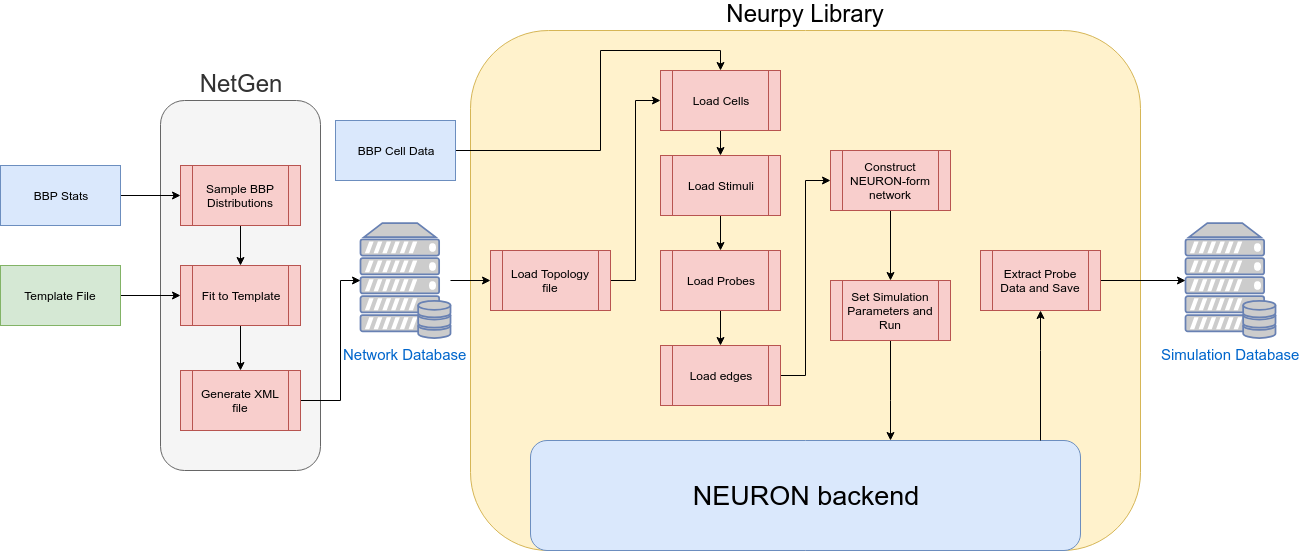
\includegraphics[width=\textwidth]{SimFW.png}
    \caption{Structure of experimental environment}
    \label{fig:nrpySimFw}
\end{figure*}
At this point, all the components of the simulation framework have been defined. An overview of the entire process is shown in Figure \ref{fig:nrpySimFw}. The general flow of this process is from left to right. On the left we begin with the network generator. We feed the statistical data on the cell-to-cell pathways from the BBP along with a topology template into NeurGen. Within NeurGen we can then generate a large number of unique individual networks, which we store as the "Network Database". After the database of networks has been created, we can begin feeding this into the Neurpy library, file by file. For each network file, Neurpy loads the specified cell model data from the BBP, loads and connects the required stimuli, loads and connects the required measuring probes, and finally connects the cells together to form the in-session network. Following this, the session simulation parameters are set (timestep, simulation length etc.) and Neurpy instructs the NEURON backend to begin the simulation. After the simulation has completed, all data is extracted from the probe vectors, converted and concatenated in a Python-native format, before being written to the disk. By repeating this for all network files, we create the "Simulation Database" which contains the voltage-vs-time data for each probe in each simulation, which we can then use for analysis.\\
\section{EXPERIMENTAL METHODOLOGY}

\subsection*{Simulation Dataset}

The cortical networks for the study of the link-level parameters between the neuronal cells were generated using the NeurGen script described above. A simple 2-cell topology template was passed to the generator which defined a network of 2 cells (with no constraint on cell type), a stimulus on the "head" node, and a probe on each node. As this portion of the investigation deals with the link-level parameters between any 2 cells in the cortical circuits, there was no need for a topology more complex than 2 cells. The simulator script was then modified slightly so that after the loading of each topology (but prior to the running of the simulation) some parameters of the link were forcibly varied. These parameters included the link delay and weight, the distance between the nodes, as well as the interval, delay, weight, and symbol probability of the stimulus. These variations were output to a separate "metadata" file for each simulation such that they could be used in the analysis to find correlations in the data. After this, the network was simulated with a simulation length of 1000ms.

\subsection{Train Discretisation and Probability Analysis}
The first step in the probabilistic analysis is to discretise the voltage-time spike trains into a binary series, similar to the process followed in \cite{spikeTrainInfo}. In our case, the process undertaken was as follows:
\begin{enumerate}
    \item Threshold the spike-train - values above $V_{thr}$ are set to 1, all other values set to 0
    \item Subdivide the thresholded train into a number of windows of length $L_{w}$
    \item Check for the presence of a spike within the window, set the window-value to 1 if found, 0 otherwise
    \item Convert the window-interval values into a binary sequence
\end{enumerate}
The binary output sequence of this process represents the symbol of the system; in this case our symbol is 1 bit and so our symbol set can be described as $S=\{s_{1}=0, s_{2}=1\}$. Here we can calculate the binary sequence from the head cell (which we can represent as a random variable $X$) as well as from the tail-cell (represented as random variable $Y$) With this in mind, we can use the previously-described equations for calculating the entropy of the head-cell and mutual information of the cortical link. The probability mass function (PMF) of both X and Y (that is, $P(X)$ and $P(Y)$) can be calculated from their respective binary sequences. We can then apply various forms of Baye's rule, along with further analysis of the two binary sequences, to obtain the joint PMF ($P(X,Y)$) and the conditional PMF ($P(X|Y)$) for use in the calculation of the mutual information of the cortical link.

\subsection{Delay Estimation}
For the estimation of the cortical link, we employ a simple cross-correlation analysis. The cross-correlation function describes the relation between two signals across a series of time shifts, and is described by
\begin{equation}
    \label{eq:xcorr}
    r_{xy}(l) = \sum_{n=-L}^{L-1}x(n)y(n-l)
\end{equation}
where $r_{xy}$ is the cross-correlation of $x$ and $y$ and L is the number of lags (time shifts) to calculate for in the positive and negative direction. Conceptually, a spike in the head cell should result in a spike in the tail-cell separated roughly by the delay as the spike crosses the synaptic connection. As a result, we should find a peak in the cross-correlation between the voltage measurements of the two cells as the time shift approaches the delay since at this time-shift the signals should be relatively well correlated.\\
While this approach is quite basic and may not be overly accurate, it is a first step in expressing the characteristic function of the delay in the neuronal link, which is an important concept when applying network tomography to estimate link-level delay, as discussed in \cite{netTomFour}.\\

\subsection{Cell Classification}
As previously mentioned, the Linear-Nonlinear-Poisson (LNP) cascade model can be used to model and characterise the response of a neural cell. Generally, this is computed using the spike-triggered-average (STA) of the stimulus sequence however this approach is more appropriate when dealing with external stimuli such as a spatio-temporal screen, such as discussed in \cite{lnpInBrain}. For this reason, the FIR-filter estimation method described in Equation \ref{eq:estFilter} was used to reduce the dimensionality of the measured features. \\
To investigate the classification of neuronal cells and to train the support-vector machine (SVM) classifier, MATLAB was used. Matlab is a tool widely used for the numerical analysis of data and offers a wide range of additional add-ons, a large community backing, and an efficient backend. One of the add-ons available in Matlab is the \emph{Classification Learner}. This is a tool that takes a dataset as input, requests the specification of the features and classes in the dataset, and then quickly trains a number of different classifiers against the data, reporting the individual classifier accuracy, confusion matrix, and receiver-operating-characteristic (ROC) curve. This tool is therefore very useful for quickly getting an idea of how the different forms of classifier are dealing with the given features and classes. \\

We have previously discussed how each of the cells in the dataset has been classified by the BBP; that is, each cell has an associated layer, m-type, and e-type. As there are over 1000 individual cell models, it is unlikely that a classifier will be capable of gaining any form of functional accuracy in directly classifying the exact cell type. For this reason, the classification of a given cell was broken down in the classification of each of its constituent components, i.e. 3 separate classifiers were trained to estimate the cell type. The first classifier estimates the layer to which the cell belongs based on the filter coefficients extracted through equation \ref{eq:estFilter}. The second classifier estimates e-type based on the filter coefficients as well as the output of the first classifier (the layer estimation). The final classifier estimates m-type based on the filter coefficients, the estimated layer, and the estimated e-type. In this format, each classifier is only estimated against 5, 11, and 24 classes respectively. The other benefit of this approach is that the output of one classifier can be fed into the next, which allows the classifier to take into account the associated probability of one class leading to another, for example it might be more likely that layer 1 neurons contain more pyramidal m-types.\\


\section{RESULTS}

\subsection*{Delay Estimation}
As stated previously, the analysis of the link-level details of a synaptic connected was done through the simulation of around 10,000 simple 2-cell networks. This results in the production of sets of voltage data for each simulation, one from the "head" cell and one from the "tail" cell. As the output of one cell is acting as the stimulus to the other, the spike trains from the simulations tend to be correlated. The output plots of a number of a few of these simulations is shown in Figure \ref{fig:sample2CellPlots}. In these sample plots, the source-destination spike correlation is clear to see as a spike in the pre-synaptic cell often results in a spike in the post-synaptic cell. As well as this, the plots indicate a slight delay between the source and event spikes.
\begin{figure}[ht]
    \centering
    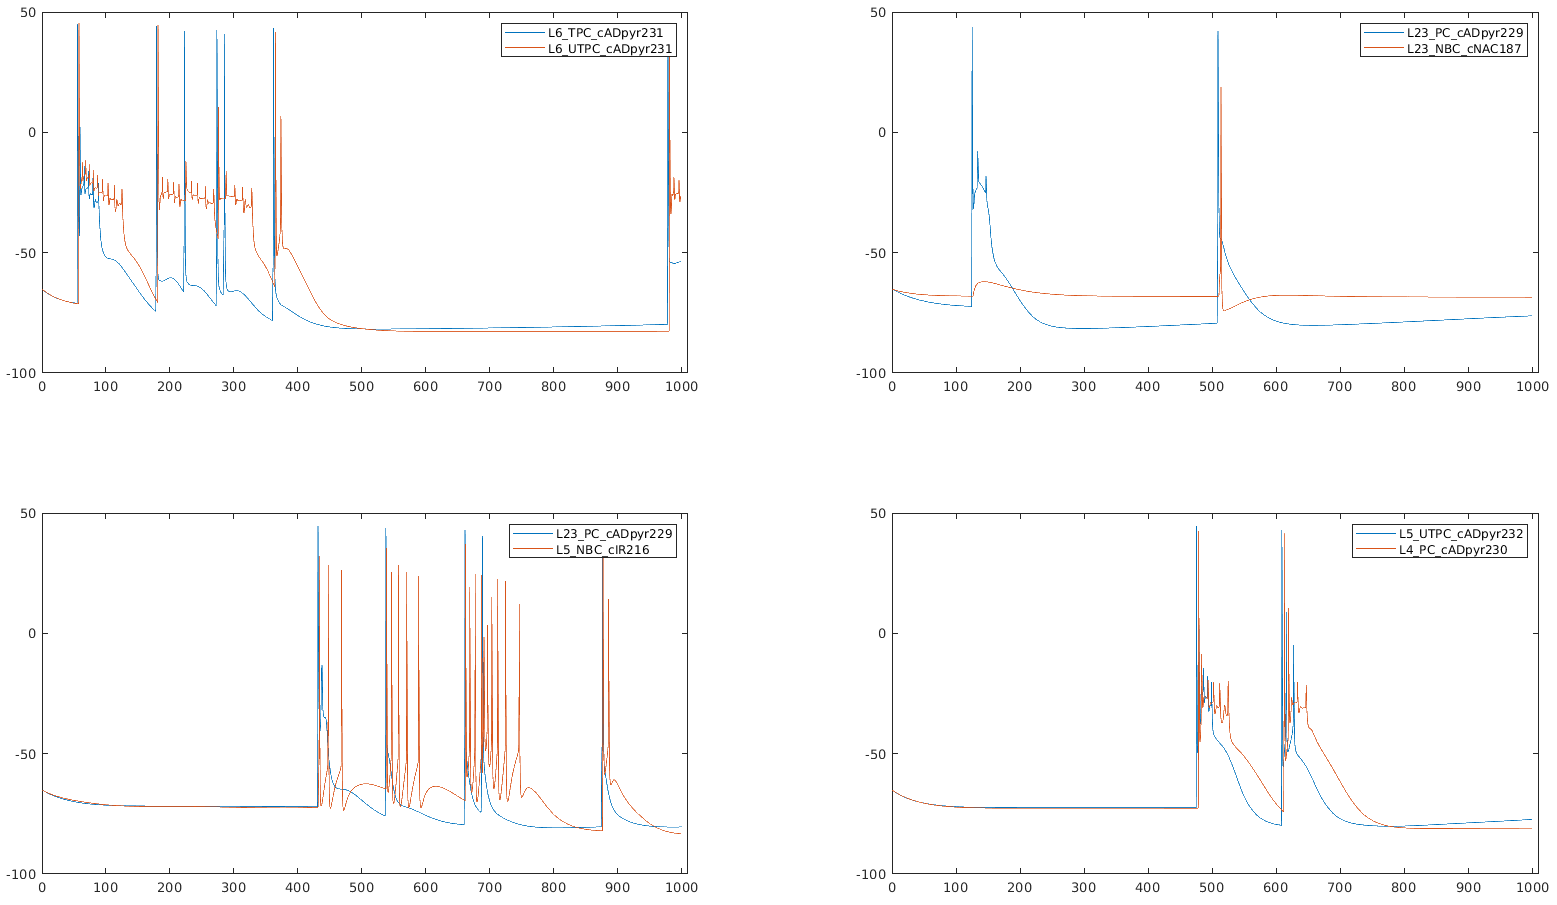
\includegraphics[width=0.48\textwidth]{2cellComp.png}
    \caption{Comparison of 2-cell network outputs. Head cell in blue, tail cell in orange. Cell-types shown in each subplot's legend}
    \label{fig:sample2CellPlots}
\end{figure}

\par

Following the collection of the simulation data, analysis was done on the estimation of the link delay through the use of the cross-correlation between the two measured voltage plots. This was implemented by loading the two cell voltage series, and using the Matlab \emph{xcorr()} function to get the cross-correlation of the two series to a specified number of lags. Next, we find the closest positive peak in the cross-correlation using the \emph{findpeaks()} function. This function finds the local maxima in a series which are the portions of the plot where the first derivative is 0 and the second derivative is negative (concave-down). By making the assumption that the first local maxima represents the delay, we can obtain a simple estimate of the link delay. Figure \ref{fig:sample2CellCorrPlots} shows a number of plots representing this delay estimation. Each subplot shows the cross-correlation of the 2 signals at a number of lag values from -12ms to +12ms, along with the location of the estimated link delay (i.e. the location of the first positive peak) and the location of the actual link delay (as specified by the \emph{delay} parameter in the associated \emph{NetCon} object.\\

\begin{figure}[ht]
    \centering
    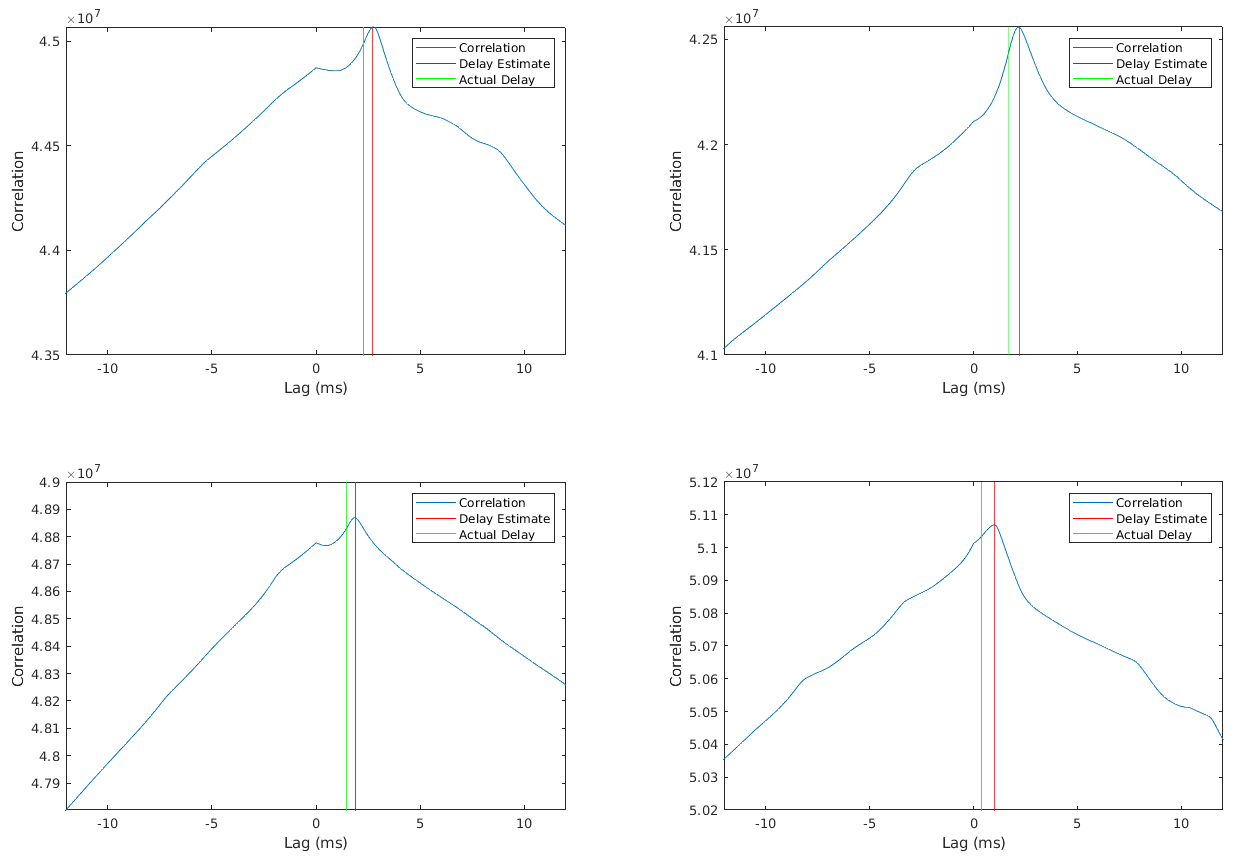
\includegraphics[width=0.48\textwidth]{2cell_Corr.png}
    \caption{Comparison of 2-cell cross-correlation with delay estimate. Cross-correlation shown in blue, estimated delay as a vertical red line, actual delay as a vertical green line}
    \label{fig:sample2CellCorrPlots}
\end{figure}

With this method of delay estimation, the estimator was run against all the simulated networks (N=10,000) and the correlation between the estimated delay and the actual delay was analysed. First, the estimations of 0ms were removed, as this was the "error value" returned by the estimator when it was unable to determine the actual delay (possibly due to a lack of spike-data in the simulation). A linear model was then fit to the data in order to determine the correlation between the estimation and the actual delay. A scatter-plot of the estimation and actual delay is shown in \ref{fig:2CellDelayLFit} along with the least-squares linear fit and associated R-squared score. The mean-squared error of this linear model was 1.0881.
\begin{figure}[ht]
    \centering
    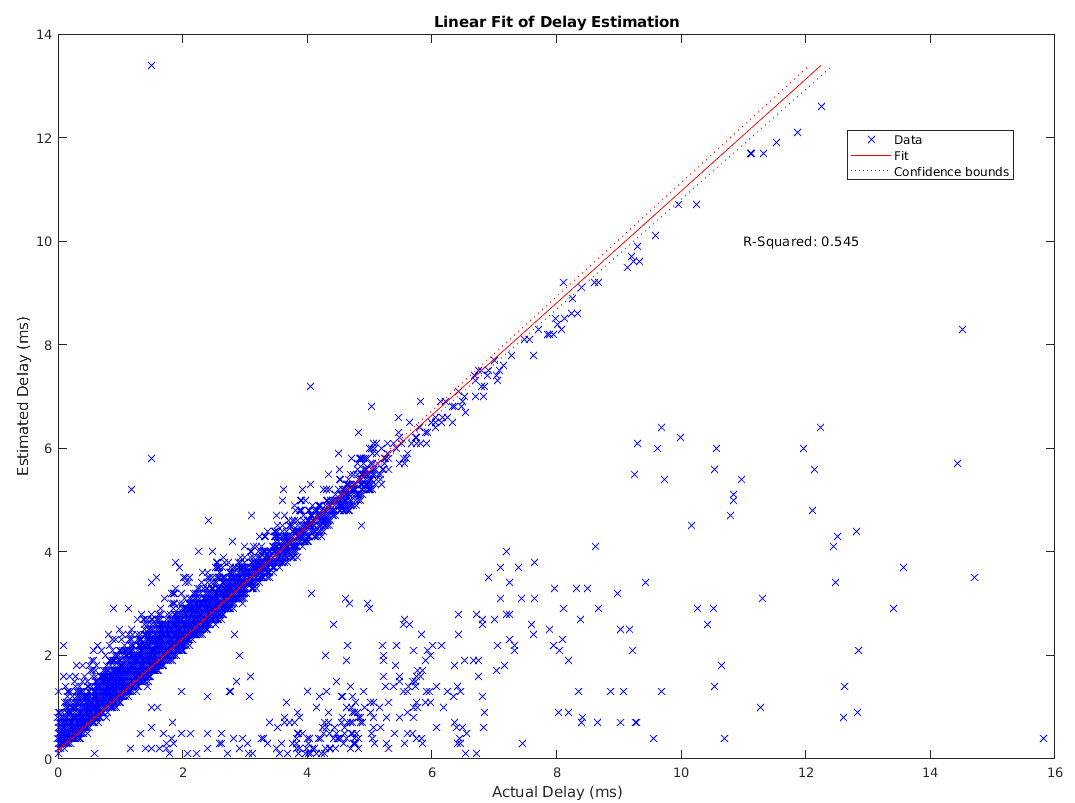
\includegraphics[width=0.48\textwidth]{delayFit.png}
    \caption{Correlation of delay estimate vs actual delay with least-squares linear model and associated R-squared score}
    \label{fig:2CellDelayLFit}
\end{figure}

\subsection*{Entropy and Mutual Information}
As discussed previously, the entropy of the cells is calculated by discretising the spike train and treating it as though the spikes represent a single binary symbol. The process for was again implemented in Matlab. Using the symbol sequence it is then possible to apply the definition of mutual information in Eq. \ref{eq:mutualInf} to determine the entropy of the individual cells, and the mutual information of the cell-to-cell connection. As well as this, we can use the delay estimation model described above, which allows us to shift the spike train of the "tail" cell such that the spike-response should be instantaneous. This is done to investigate whether or not adjusting for the delay in the link will effect the calculated mutual information.\\
The probability-mass function (PMF) of the calculated single-cell entropy is shown in Figure \ref{fig:cellEntPmf}. The majority of the cells have an entropy of below 0.4 bits/symbol, with a continuously decreasing proportion of the cells having an increasing entropy. The PMF of the calculated mutual information is shown in Figure \ref{fig:mutualInfoPmf}. We can see that the mutual information of the networks is well-distributed, with a mean of around 0.5 bits. Of note here is that the effect of shifting the spike-train based on the delay estimate has little to no effect on the distribution of the mutual information. \\

\begin{figure}[ht]
    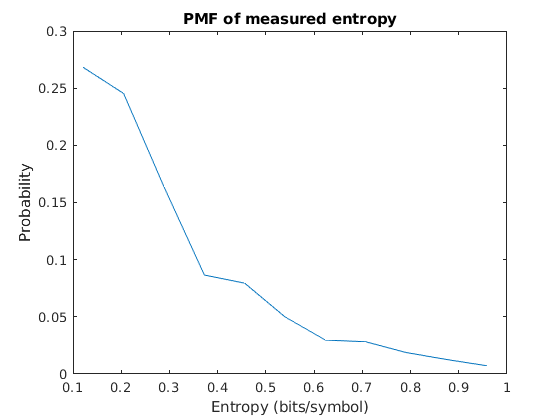
\includegraphics[width=0.48\textwidth]{entropyPmf.png}
    \caption{PMF of calculated single-cell entropy based on output spike trains}
    \label{fig:cellEntPmf}
\end{figure}

\begin{figure}[ht]
    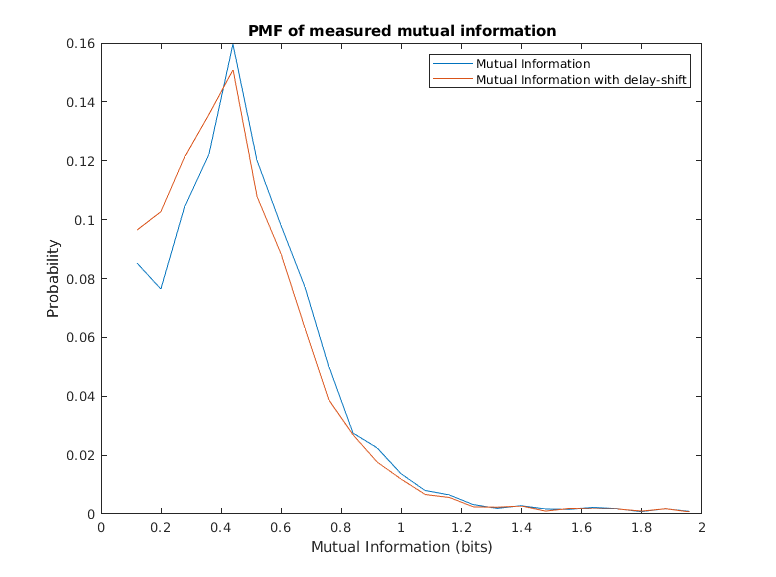
\includegraphics[width=0.48\textwidth]{mutualInfo_pmf.png}
    \caption{PMF plots of calculated mutual information for the measured spike-train (blue) and the delay-estimate shifted spike-train (orange)}
    \label{fig:mutualInfoPmf}
\end{figure}


We next look at the possible factors that may have an effect on the mutual information. We can plot a number of scatter-graphs to visually represent any correlations in the data, as shown in Figure \ref{fig:mInfoCorrGraph}. In this figure, we can examine any correlation between the mutual information and the number of synapses in the connection, the delay in ms of the link, the weight of the link, and the distance between the 2 cells in the network. We can see that there is no obvious correlation between any of the link-level parameters and the mutual information of the network.\\
\begin{figure}[ht]
    %\centering
    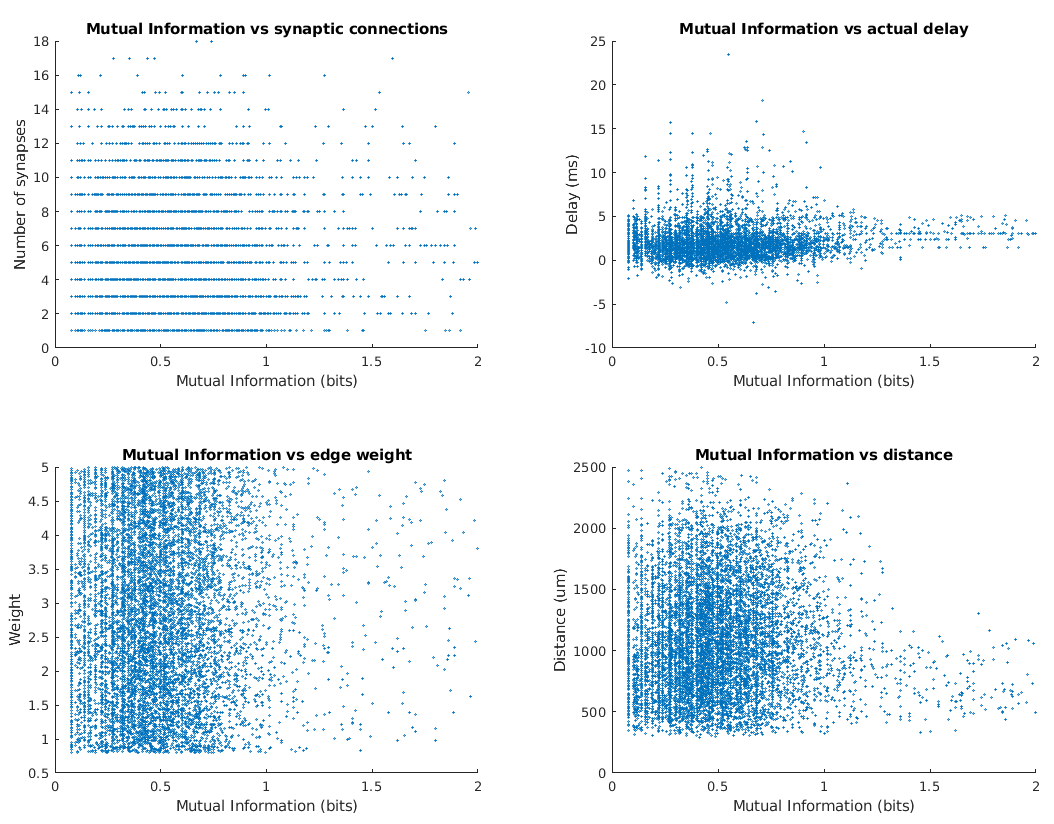
\includegraphics[width=0.48\textwidth]{minfoCorrPlot.png}
    \caption{Scatter plots of measured mutual information vs number of synapses, edge delay, edge weight, and distance between the cells.}
    \label{fig:mInfoCorrGraph}
\end{figure}
While there is no obvious correlation between any single parameter and the mutual information, these 2-d plots do not take into account all of the link parameters at once; that is, it could be that correlation could be found by analysing the dimension-space made up of all measured parameters. This can be done using a linear model, as used to determine the correlation in the delay estimate. In this case, we use multiple predictor variables (the link parameters) and a single response variable (the mutual information). This model is shown in Figure \ref{fig:lmInfo}. With an R-squared score of 0.034, it is clear that there is no correlation between the network parameters and the mutual information of the neural link.
\begin{figure}[ht]
    \centering
    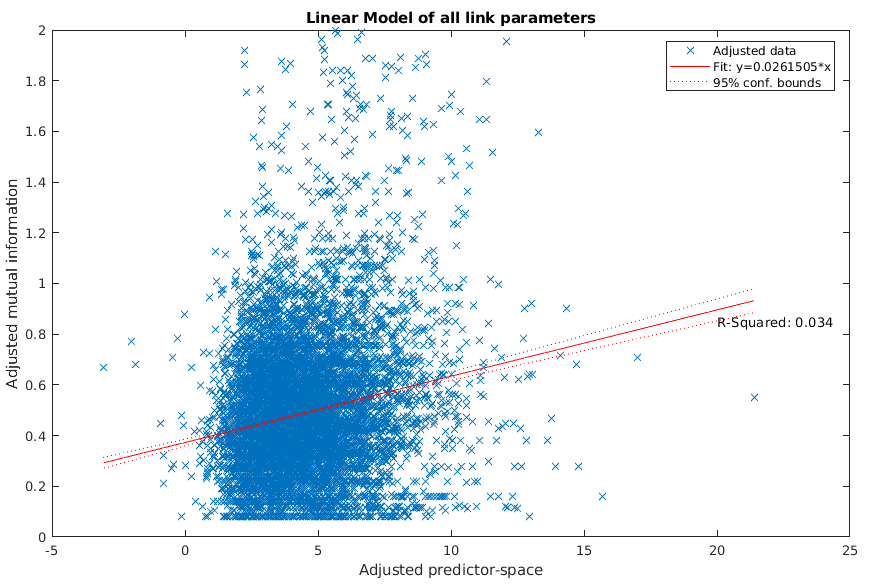
\includegraphics[width=0.48\textwidth]{lmMinfo.png}
    \caption{Linear fit of all network parameters to predict mutual information}
    \label{fig:lmInfo}
\end{figure}


\subsection*{2-Cell Classification and Model Training}
% \begin{itemize}
%     \item Spike train figures showing the difference in impulse response between cells
%     \item Some figures of the LNP estimation and associated coefficients
%     \item Some scores on the separation of the filter coefficients between cell classes
%     \item Confusion matrices and different model metrics for the classification models, and the differences in the analysed algorithms (GMM, SVM, NN etc)
% \end{itemize}
% TODO: above

In Figure \ref{fig:sample2CellPlots} a number of spike-trains from different cell types were shown. Referring back to this, it is clear that different cells respond different to stimulus, with the output spike train differing in intensity (frequency of spikes) as well as in the "settle-down" period after a spike was triggered (i.e. the fall-time response of the membrane voltage). It is these differences that we attempt to characterise through the use of the linear-filter portion of the linear-nonlinear-Poisson (LNP) cascade model.\\
The first step in this process is to simulate a number of 2-cell networks again in order to generate test data. In this instance, the "head" cell acts only as a stimulus generator, and we treat the soma-membrane potential of this cell as the "input" voltage to the linear system described in \ref{eq:firLinSys}. In order to limit the number of variables in this investigation, the type of cell used as the head cell was constant across all simulations (layer 1, DAC m-type, bNAC e-type) while the "tail" cell was treated as the cell-under-test and so was varied between simulations. As well as this, variations in link-level parameters (number of synapses etc.) were kept to a minimum to reduce the number of variables. A large number of networks were generated (N=30,000) in order to produce a dataset of sufficient size for classifier training.
Following simulation and prior to training the classifiers, the filter estimation step described in equation \ref{eq:estFilter} was applied to extract the filter coefficients as features from the cell-response data. Figure \ref{fig:sampImpRes} shows the filter coefficients (FIR impulse response) of 4 different cells, with a filter-order of 64. It is clear from this diagram that the impulse-response estimation of the neuronal cell is capable of differentiating between the cell types. Using these estimated filter coefficients, we are now able to begin training the classifiers.
\begin{figure}[ht]
    \centering
    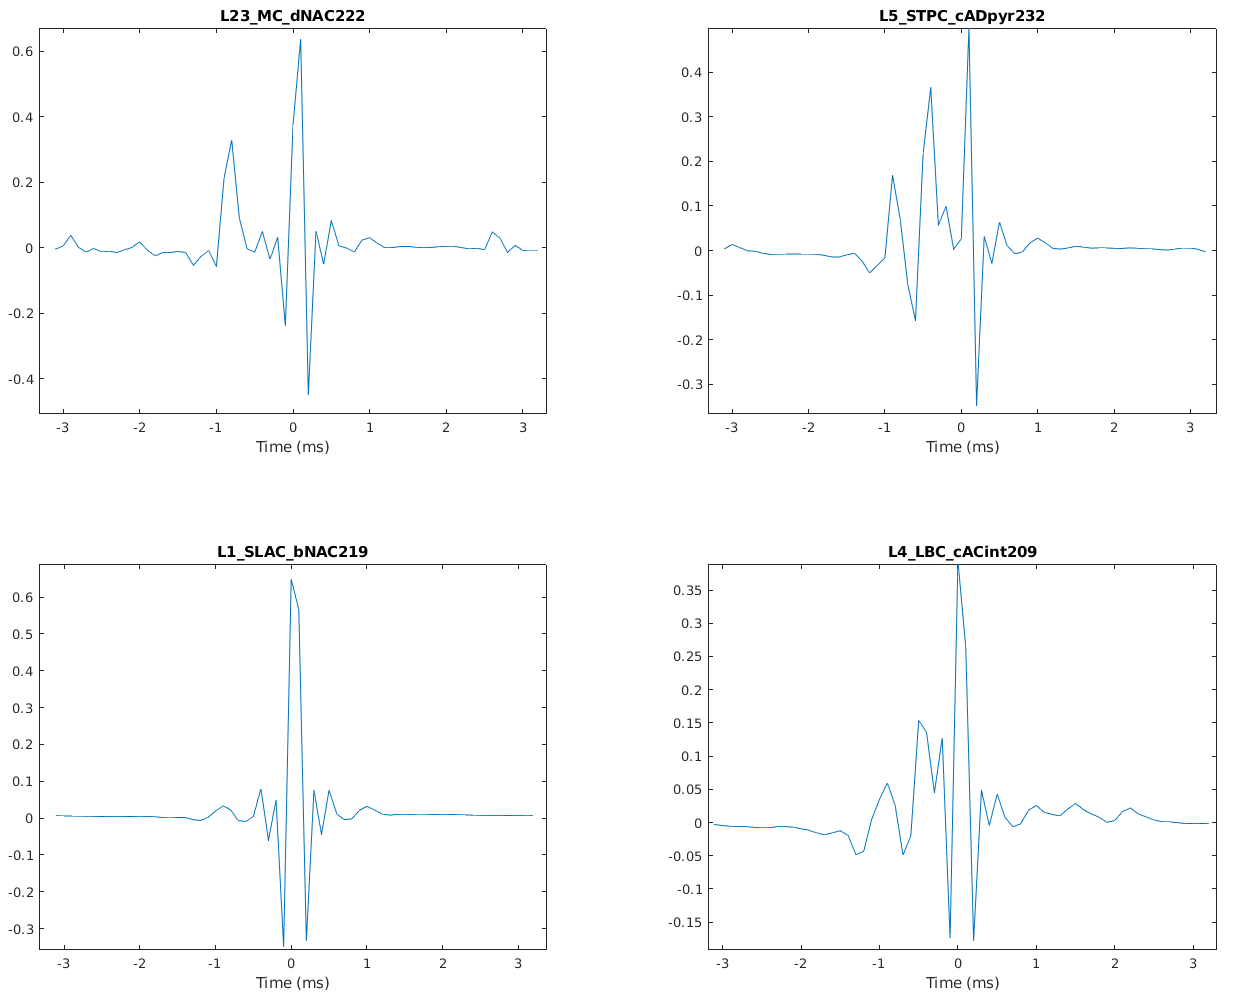
\includegraphics[width=0.48\textwidth]{sampImpRes.png}
    \caption{Sample impulse-response characterisation of different cells}
    \label{fig:sampImpRes}
\end{figure}

\par

Using the previously discussed \emph{Classification Learner} tool in Matlab, we can quickly train and compare a set of different classifiers, inspecting the accuracy, confusion matrix, and receiver-operating characteristic (ROC) curve for each. The first classifier to investigate is the layer classifier, which takes the estimated filter coefficients as input, and attempts to estimate what layer the characterised cell belongs to. We use this tool to train and analyse an SVM-based classificaiton system\\
The performance of the classifiers are shown in the following tables. In each table, we compare the performance of the different classification algorithms (Decision Tree, SVM etc.) in the classification of the separate cell sub-group types (layer, m-type, e-type). For each classifier we state the corresponding accuracy. The accuracy is calculated as the ratio of correct estimations versus incorrect estimations. We also state the "factor improvement" of the classifier. This is calculated as the factor by which the classifier improves over the equivalent accuracy of random guessing in the classification space. For example, with 5 layer classes the equivalent "random guess" accuracy is 20\%, and so a trained classifier with accuracy of 40\% would have a factor improvement of 2. \\

Table \ref{tbl:layerClassifierPerf} shows the performance of the classifiers in the prediction of cell layer-type, table \ref{tbl:mtypeClassifierPerf} for m-type prediction, and table \ref{tbl:etypeClassifierPerf} for e-type prediction. In every case, the SVM classifier has the highest accuracy, with the NN being slightly behind. Of the tree-based classifiers, interestingly the decision tree based classifier has a consistently higher accuracy than the random forest classifier, despite the latter being a variant of the former. 


\begin{table}[h]
    \centering
    \begin{tabular}{|c||c|c|c|c|}
        \hline
        Classifier & Decision Tree & Random Forest & SVM & NN\\
        \hline\hline
        Accuracy & 52.2\% & 41.43\% & 62.5\% & 60.98\%\\
        \hline
        Factor Improvement & 2.61 & 2.07 & 3.13 & 3.05 \\
        \hline
    \end{tabular}
    \caption{Performance of different algorithms at classifying cell-layer (5 classes, 20\% equivalent random guessing accuracy)}
    \label{tbl:layerClassifierPerf}
\end{table}

\begin{table}[h]
    \centering
    \begin{tabular}{|c||c|c|c|c|}
        \hline
        Classifier & Decision Tree & Random Forest & SVM & NN\\
        \hline\hline
        Accuracy & 42.6\% & 35.07\% & 63.7\% &57.99\%\\
        \hline
        Factor Improvement & 10.65 & 8.77 & 15.93 &13.92\\
        \hline
    \end{tabular}
    \caption{Performance of different algorithms at classifying cell m-type (25 classes, 4\% equivalent random guessing accuracy)}
    \label{tbl:mtypeClassifierPerf}
\end{table}

\begin{table}[h]
    \centering
    \begin{tabular}{|c||c|c|c|c|}
        \hline
        Classifier & Decision Tree & Random Forest & SVM & NN\\
        \hline\hline
        Accuracy & 63.8\% & 54.47\% & 75.3\% &73.94\%\\
        \hline
        Factor Improvement & 8.93 & 7.63 & 10.54 &10.35\\
        \hline
    \end{tabular}
    \caption{Performance of different algorithms at classifying cell e-type (14 classes, 7.143\% equivalent random guessing accuracy)}
    \label{tbl:etypeClassifierPerf}
\end{table}

\par

Another set of results that are often used to quantify the performance of a classifier is the class precision and the class recall. The class recall is calculated per-class as the ratio of correct predictions of a class versus the number of observations of that class. The class precision is again calculated per-class as the ratio of correct predictions of a class versus the overall number of the classifier estimated that class.  As these metrics identify the performance of the model on a class-by-class basis, it results in a large number of individual values to compare. When we consider that we are comparing 3 estimator groups with a relatively high number of classes per group (5 for layer estimator, 25 for m-type, and 14 for e-type), as well as the fact that each estimator group must be compared against 4 different classification algorithms, it becomes difficult to critically compare the performance of each individual class. In general, however, when analysing such metrics from single classifier, a \emph{confusion matrix} is used. The confusion matrix of the SVM-based layer estimator is shown in Figure \ref{fig:svmConfMatLayer}. The confusion matrix tabulates the estimations of a given classifier as a grid of "True Class" versus "Predicted Class". In this way, it can show how often an observation of a given class is estimated as belonging to some other class. As such, the diagonal (shown as green in the confusion matrix figure) shows the proportion of the correct predictions in the validation set (where true class equals predicted class). The right hand bar shows the proportional difference of the \emph{true positive rate} and the {false negative rate}. This true-positive rate is equivalent to the class recall.\\
While the confusion matrices for every single classifier investigated in this study are not included, the relative proportions between them tend to be similar (i.e. very high prediction accuracy between layer 1 and layer 6, with reduced accuracy in the intermediate layers).

\begin{figure}[ht]
    \centering
    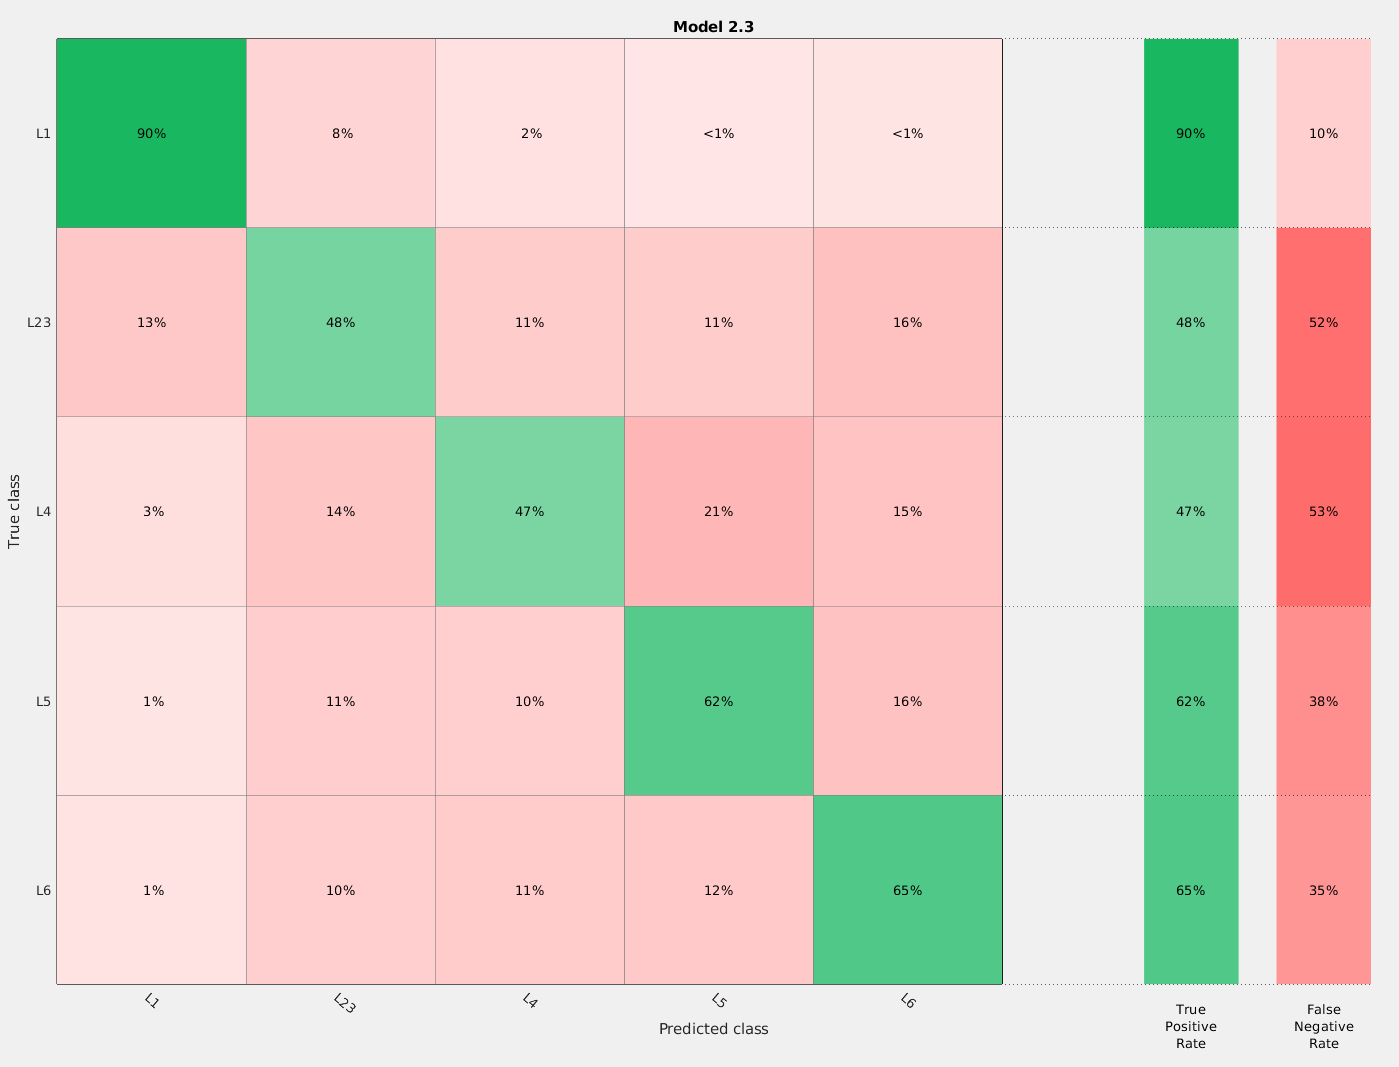
\includegraphics[width=0.48\textwidth]{svmLayerConf.png}
    \caption{Confusion Matrix of SVM layer-classifier}
    \label{fig:svmConfMatLayer}
\end{figure}



\subsection*{Network Tomography for Cellular Classification}
% \begin{itemize}
%     \item Figures of 4-leaf networks
%     \item Metrics in the reconstruction of these networks
%     \item Some figures showing the estimated network reconstruction vs actual network etc.
% \end{itemize}

As the SVM classifier had the best performance during training, this is the model that was applied in the reconstruction of the 4-leaf star networks. The process here was similar to the previous experiments: a number of unique networks were generated, simulated, and their data-points measured and analysed. In this case, the networks generated were of the 4-leaf star topology previously discussed. The central node was constrained to be of the same layer 1, DAC m-type, bNAC e-type cell type used in the training of the models, while the star cells were varied. For each measurement from the soma-membrane of a star node, the characteristic filter was estimated using the same process discussed previously, and the filter coefficients were passed through the pre-trained classifiers.

\par
The performance results of the topology reconstruction are shown in Table \ref{tbl:wholeClassifierPerf}. Here, we tabulate the accuracy of the classifier chain in estimating layer, m-type, and e-type groups, as well as the "whole-cell" classification accuracy. We define the whole-cell accuracy as the the cases where all three sub-groups were correctly estimated. Evidently, the factor-improvement for the whole-cell prediction is significantly higher than for any other group, while the sub-group accuracy is quite similar to those in the 2-cell networks.

\par

Figure \ref{fig:4CellRecon} shows a sample reconstruction of a 4-leaf network from probe measurements. The left side of the figure represents the network as it was simulated, with probes at the network endpoints and a stimulus on the central node, along with the actual cell types of the leaf nodes. The right side of the figure shows the reconstructed topology based on the cell-type estimations from the SVM classifier chain. 

\begin{figure}[ht]
    \centering
    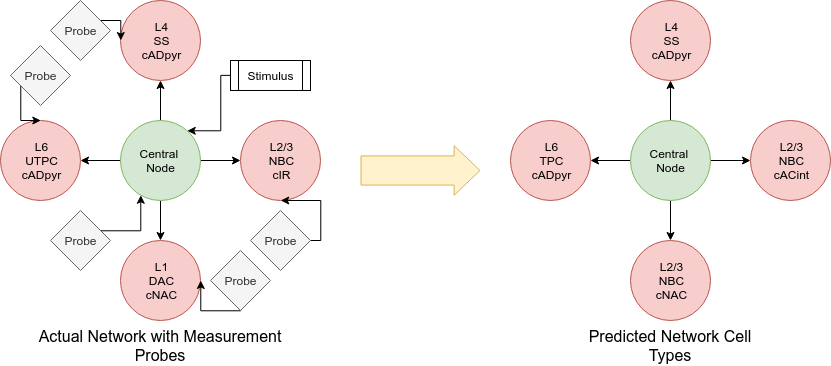
\includegraphics[width=0.48\textwidth]{4cellTopRecon.png}
    \caption{Sample reconstruction of network}
    \label{fig:4CellRecon}
\end{figure}

\begin{table}[ht]
    \centering
    \begin{tabular}{|c||c|c|c|c|}
        \hline
        Prediction & Layer & m-type & e-type & whole-cell \\
        \hline\hline
        \# classes & 5 & 25 & 14 & 1750\\
        \hline
        Equiv. random guess accuracy & 20.0\% & 4.0\% & 7.143\% & 0.0571\%\\
        \hline
        Classifier accuracy & 61.82\% & 56.34\% & 64.62\% & 36.23\%\\
        \hline
        Factor improvement & 3.091 & 14.085 & 9.05 & 634.5\\
        \hline
    \end{tabular}
    \caption{Performance of 4-leaf star topology reconstruction}
    \label{tbl:wholeClassifierPerf}
\end{table}


\section{DISCUSSION}
\subsection*{Delay Estimation}

The delay estimation has proven to be quite accurate considering the relatively simple concept it is based on. While the estimated delay tends to be higher than the actual delay, the proportional difference between the two seems to be relatively constant meaning that a clear correlation can be seen, and that a simple linear model can fit with a decent R-squared score. This nearly constant difference between the estimation and the actual value can be explained by the nature of the simulation; the "ground truth" value taken as the network delay is the corresponding parameter applied to the \emph{NetCon} object connecting the two cells, while the measurements we take come from the soma of the two cells. This means that any delay we observe is from the delay of signal propagation through the axom of the presynaptic cell, through the NetCon object, across the synapse, and then through the dendrites of the post-synaptic cell. This means that any observed delay would be higher than the delay of just the NetCon object, which is supported by our data.\\
Another point of consideration in the delay estimation is that the estimator was not always able to predict a delay. This in general is due to the lack of peaks in the cross-correlation, which in turn may be caused by a lack of spikes in one or both of the voltage measurements possibly caused by a lack of synaptic connections. In these cases, the estimator returns a delay of 0ms. For this reason, any estimations of 0ms delay were simply removed from the dataset as they were assumed to have been caused by an invalid simulation.\\
Future work in this area could take the whole delay path into account when forming the ground truth in the simulated network to verify the hypothesis that the estimation discrepancy is caused by this inaccurate ground truth. On top of this, the current model is quite simple in design and so could be improved upon to increase the robustness of the estimator to edge-cases where simple cross-correlation is not sufficiently accurate.

\subsection*{Mutual Information}

While the distribution of the measured mutual information in the simulation dataset does tend to follow a normal-like fit, it is clear from the various scatter plots that there is no correlation between the various link-level parameters between the cells and the discrete-memoryless model applied to the discretised spike trains. This lack of correlation is confirmed by the linear model which was "fit" to each of the link parameters, indicating a very low correlation with an R-squared score of only 0.03. This suggests that the application of the information model commonly used in digital systems is not sufficient to describe the information carried between cells through synaptic connections, possibly due to the fact that the transmission of a signal between two neurons is not entirely memoryless as the synapse has a refactory period during neurotransmitter reuptake. This could also be explained by a lack of sample data, as previous work done in this area has suggested that the accurate prediction of the entropy and mutual information of these links relies heavily on the size of the dataset, in particular of the length of the simulation and the number of spikes observed \cite{spikeTrainInfo}. As a result of this, future work in this area could investigate the effect of the simulation length and the activity within the simulation on the correlation between the calculated mutual information and the link parameters.\\
As well as this, other models could be applied in this domain to find the above parameter-information effect; for example, the calculation of upper and lower bounds on the mutual information as well as different approaches to the conversion between measured spike-trains and symbol sequences could be applied \cite{spikeTrainInfo}.

\subsection*{Classification}
The classification of cell types from measured membrane potential has shown promising results, with relatively high accuracy considering the high number of classes to which the models were estimating. Evidently, the SVM-based classifier had the highest level of accuracy, with the artificial neural network being close behind in performance. This was surprising, as neural networks are widely used for high-order classification problems. It is possible, however, that the close level of accuracy between the two is indicative of the limit of the features on which we are predicting and that the level of information that the features hold does not allow for accuracy above this level. This is supported by the fact that tweaks to the classifiers' parameters (i.e. kernel size in SVMs and hidden-layer size in the neural networks) did not have any noticeable effect on the accuracy, indicating that they are close to maximising the classification based on these features. Future work in this area could therefore look at the extension of the feature-space. For example, while we based the feature extraction on the characterisation of a cell from the LNP cascade model, we ignored the nonlinear transformation component. Taking this component into account could improve the accuracy of the classifiers. Another consideration to be made here is the size of the linear filter used as the characteristic features (the order of the FIR filter). A number of different filter sizes were investigated, however we found that above about 64 coefficients, the accuracy did not improve. This again indicates the limit of this feature set, which is supported by the plots of the impulse response of some of the estimated filters in Figure \ref{fig:sampImpRes}. Here we can see that the majority of the characterisation between cell types is in the central coefficients, with reduced variance as we move away from the 0-point. Increasing the order of the filter will only add detail to the two extremes of this impulse response, which adds features that seem to bare little characterising information.\\
As mentioned previously, the accuracy metric chosen to compare the classifiers does not fully indicate the performance of the model. When dealing with this form of classifier, a confusion matrix and associated class-recall and class-precision metrics can give a much more informative idea of the efficacy of the estimator. In this case, however, the amount of individual values that would need to be compared between the three sub-groups (each with varying amounts of classes) and the 4 classification algorithms makes it unfeasible to directly compare the models in this way. With that in mind, it was found that the class recall and class precision were quite similar between the 4 classification algorithms meaning that directly comparing the accuracy of the models can give a good idea of the comparative performance.\\
Another consideration here is with the "factor improvement" metric, taken as the proportion improvement of the model's accuracy versus the equivalent accuracy of randomly guessing with the class-space. The equivalent accuracy of random guessing assumes that the distribution of the classes amongst the dataset is equal, i.e. the probability of one class occurring is no higher than any other class. While this is true for the layer-group (since the dataset was constructed ensuring an equal proportion of each of the layers) it is not necessarily true for the m-type and e-type classes as some of these groups are more likely to occur than others. On top of this, the number of possible classes for the "whole-cell" type classification was taken to be the product of the number of layers, m-types, and e-types. This does not take into account that some permutations of these groups do not occur in the dataset (however they may occur in practice), and so the actual factor improvement may be lower than observed. With this in mind, however, it is worth noting that the distributions of these classes are not significantly skewed in any single direction, and so while not fully indicative of the performance, the factor improvement does show the general trend of the estimators.\\
Keeping these considerations in mind, it is clear that the classifiers show a positive trend in cell-type estimation. In all cases, the decision tree classifier performed better than the random forest classifier, which is surprising as the random forest algorithm is a variation of the decision tree algorithm which should have higher performance. This could be explained by the fact that decision tree classifiers tend to overfit to the dataset, which might result in higher training accuracies.\\
The classifier with the highest performance in all cases was the SVM-based model. In classifying the layer type, the SVM model was capable of achieving 62.5\% accuracy, a factor improvement of 3.13 over random guessing. By looking at the confusion matrix for this classifier in figure \ref{fig:svmConfMatLayer}, we can see that the classifier has very good performance in classifying between layer 1 and layer 6 with close to 100\% accuracy between these classes where only 1\% of layer 6 cells were predicted as layer 1, and less than 1\% of layer 1 cells were predicted as layer 6. The overall accuracy decreases as the intermediate layers are added, with the worst performing component being incorrectly predicting a layer 4 cell as layer 5 21\% of the time. It is evident, therefore, that the highest degree of separation using the FIR-filter estimation is between layer 1 and layer 6.\\
In the reconstruction of the 4-leaf topology through endpoint measurements using the trained SVM classifier, the individual sub-group accuracies tend to reflect those of the 2-cell networks with a layer-estimation accuracy of 61.82\%, an m-type accuracy of 56.34\%, and an e-type accuracy of 64.62\% representing a factor improvement of 3.09, 14.09, and 9.05 respectively. The interesting result in this investigation, however, is the whole-cell estimation (where each of the individual sub-group estimators were correct) with an overall accuracy of 36.23\% and a factor improvement of 634.5. As well as this, looking at the sample reconstruction in Figure \ref{fig:4CellRecon}, it is clear that the classification model is not always correct, however incorrect estimations are often with very similar classes such as where the UTPC m-type is estimated as a TPC m-type.\\
There are a number of areas that could be worked on in future to extend the investigation of this domain. For example, to estimate the equivalent FIR filter we use both the input and the output voltage measurements, however the response of a cell is really effected only by signal impulses. Therefore, it may not be required to use the input spike train at all. Instead, the input impulse train could be estimated from the output spike train (i.e. areas where a series of spikes start could be where the cell received an impulse), and the equivalent impulse response could be determined from this. In this way, only the output of the cell would need to be measured. This would also help with the classification of more complex networks where the proportional number of measurements versus the number of cells is greatly reduced.\\
Another point that could be investigated in future work is in the variation of the central/stimulus cell. Throughout the production of our simulation database, the presynaptic cell was kept constant to minimise variables. In practice however, many different cell types may interconnect and so the ability to classify a cell regardless of the presynaptic cell type is important. Conceptually, the performance should be relatively similar as the features used in the classifiers is based on the impulse response of the postsynaptic cell, rather than the characteristics of the presynaptic cell.\\
Finally, another point of consideration for future work is in multi-path networks. In this investigation we dealt solely with single path (one cell to one cell) connections. In practice, a given cell may be stimulated by a number of presynaptic cells. This can be characterised using the LNP model by using multiple linear filters, and computing the output based on a combination of the individual coefficients \cite{lnp}. Similarly, in our study we used only excitatory synaptic connections to generate measurements with a large number of characterising spikes. Future work could therefore look at the classification of cells based on various combinations of excitatory to inhibitory connections.

\section{CONCLUSION AND FUTURE WORK}

The use of network theory in the biological domain is a field that will become increasingly important in the near future as the technology driving human-machine interfaces advances and matures. We have shown in this study that there are a number of promising applications of existing network theory to infer link-level and cell-type details. Conversely, we have also shown that some existing areas of information theory may not be applicable in this domain without adaption and research into better fitting the theory to the unique characteristics of cortical neuronal networks.\\
We have shown that the use of cross-correlation of the soma-membrane measurement of two neuronal cell can be used to estimate the link-level delay between the cells, to a relatively high degree of accuracy. Such a characterisation of the delay may be applicable in the use of more complex network tomography to identify path delay in larger neuronal networks, however more research is required into increasing the robustness of such an estimator to obtain useful results.\\
We have shown that the application of discrete-memoryless models to calculate the entropy and mutual information between two cells may not be applicable in the neuronal domain. There are a number of reasons for this, such as the differences in channel memory where the output of the discrete-memoryless model does not depend on previous inputs, whereas the neuronal channel does. Another possible explanation is the relatively short simulation length which may not contain sufficient data to obtain reliable measurements of the spike-encoded information. Regardless of the cause of the lack of correlation, it is clear that more work is needed to determine a satisfactory system that reliably models the information propagated through the cortical circuits.\\
Finally, we have shown that the classification of neuronal cell types and sub-group types is possible through the characterisation of the cell's input-output impulse response. With an average accuracy of around 58\% across the layer, m-type, and e-type class groups, the SVM-based classifier outperforms decision tree, random forest, and even artificial neural network classifiers. We have also shown that the trained classifier can then be applied in the reconstruction of the cell-types in a various forms of the 4-leaf star topology, estimating the cell-type of each leaf node to a promising degree of accuracy. While the performance was indicative of a promising trend, it is clear that more research is required to improve the robustness of this form of classification to any usable degree.\\
While the investigations carried out in this study were cursory in regard to the extremely wide scope of neurology, molecular communication, network tomography, and information theory, it is evident that the individual topics covered may be used in future for the robust and reliable network tomography of cortical neuronal molecular communication systems.

\addtolength{\textheight}{-12cm}   % This command serves to balance the column lengths
                                  % on the last page of the document manually. It shortens
                                  % the textheight of the last page by a suitable amount.
                                  % This command does not take effect until the next page
                                  % so it should come on the page before the last. Make
                                  % sure that you do not shorten the textheight too much.

\bibliography{refs.bib}
\bibliographystyle{ieeetr}

\end{document}
